\documentclass[11pt,hyperref={bookmarks=false}]{beamer}
%\usetheme{Warsaw}
\usetheme{Madrid}
\usecolortheme{beaver}
\usefonttheme{professionalfonts}
 \usepackage[usenames,dvipsnames]{pstricks}
 \usepackage{wallpaper}
 \usepackage{epsfig}
\definecolor{UniBlue}{RGB}{157,34,53}
\setbeamercolor{block title}{bg=UniBlue!70,fg=black}

\usepackage{psfrag,graphicx}
\usepackage{amsmath,amsfonts}
\usepackage{lscape}
\usepackage{array,epsfig}
\usepackage{amsfonts}
\usepackage{amssymb}
\usepackage{amsxtra}
\usepackage{amsthm}
\usepackage{makecell}
\usepackage[skip=0pt, belowskip=-10pt]{caption}
\usepackage{subcaption}
\usepackage{float}
\usepackage{multirow}
\usepackage{booktabs}
%\usepackage{subfigure}
\usepackage{eso-pic}
\usepackage{transparent}
\usepackage{graphicx}
\usepackage{tikz}
\usepackage{longtable}
\newtheorem{df}{Definition}
\newtheorem{lm}{Lemma}
\newtheorem{prp}{Proposition}
\newtheorem{sprf}{Sketch of Proof}
\newtheorem{prf}{Proof}
\newtheorem{conjecture}{Conjecture}
\newtheorem{suffc}{Sufficient Condition}
\setbeameroption{hide notes}
\newcommand{\threelinebracer}{$\left. \begin{array}{c} \\ \\ \\ \end{array} \right\rbrace$}
\newcommand{\threelinebracel}{$\left. \begin{array}{c} \\ \\ \\ \end{array} \right\lbrace$}
\newcommand{\twolinebracer}{$\left. \begin{array}{c} \\ \\ \end{array} \right\rbrace$}
\newcommand{\twolinebracel}{$\left. \begin{array}{c} \\ \\ \end{array} \right\lbrace$}
\newcommand{\bd}{\partial}

\usepackage{pgf}  
%\logo{\pgfputat{\pgfxy(-1.2,-0.2)}{\pgfbox[center,base]{\includegraphics[height=12pt, keepaspectratio]{UA_Logo_Horizontal.eps}}} }

%\usebackgroundtemplate
%{
  %  \node[opacity=0.3, at=(current page.south east),anchor=south east,inner sep=0pt] 
    %\includegraphics[width=\paperwidth,height=20pt]{UA_Logo_Horizontal.eps}%
%}

\linespread{1}
\usepackage{parskip}
%\setlength{\itemsep}{1em} 
%\addtolength{\parskip}{5pt}
\DeclareMathSizes{12}{10}{8}{6}
%  \begin{itemize}}{\end{itemize}}
% Separate slides by \begin{frame} and \end{frame}.
\title[Willingness-to-pay for Warnings]{Willingness-to-pay for Warnings: Main Tables}
\author[A. Gaduh, P. McGee and A. Ugarov]{A. Gaduh, P. McGee and A. Ugarov}
\institute[]{}
\date{\today}

\newcommand\BackgroundPic{%
\put(0,0){%
\parbox[b][\paperheight]{\paperwidth}{%
\vfill
\centering
%\includegraphics[width=\paperwidth,height=\paperheight,%keepaspectratio]{sancho.png}%
\vfill
}}}


\begin{document}
%\AddToShipoutPicture*{\BackgroundPic}

\begin{frame}
\titlepage
\end{frame}

%%%%%%%%%%%%%%%%%%%%%%%%%%%%%%%%%%%%%%%%%%%%%%%%%%%%%%%%%%%%%%%%%%%%%%%%%%%%%%%%%%%%%%%%%%%%%%%%
%%%%%%%%%%%%%%%%%%%%%%%%%%%%%%%%%%%%%%%%%%%%%%%%%%%%%%%%%%%%%%%%%%%%%%%%%%%%%%%%%%%%%%%%%%%%%%%%

\begin{frame}
\frametitle{Research Question}
\begin{itemize}
	\item How much do people value alerts (signals) about potential preventable threats?
	\item How do signal's probabilistic characteristics affect the willingness-to-pay for it and the welfare gains from using it?
	\item Applications:
	\begin{itemize}
		\item Natural disaster warnings (tornados, floods, earthquakes)
		\item Medical tests for treatable conditions
		\item Investing in research on likelihood of catastrophic events (rogue AI, global warming, pandemics)
	\end{itemize}
	\item Note: most real-life applications provide little practice with using the signal
\end{itemize}
\end{frame}


\begin{frame}
\frametitle{Overview of the Experiment}
\begin{itemize}
	\item An insurance experiment:
		\begin{itemize}
			\item Two states of the world: bad ($\omega=1$) and good ($\omega=0$)
			\item Probability of a bad state is $P (\omega=1) = \pi$
			\item Bad state $\implies$ loss of \$$L$
			\item A perfectly protective insurance can be purchased for \$$c$
		\end{itemize}
	\item Subject can purchase a signal $s$ before purchasing the insurance:
		\begin{itemize}
			\item A signal is characterized by its true-positive ($P(s=1|\omega=1)$) and true-negative rates ($P(s=0|\omega=0)$) 
		\end{itemize}
\end{itemize}

\vspace{1em}
\begin{block}{Research objective}
	How do signal characteristics affect the WTP?
\end{block}
\end{frame}


\begin{frame}
\frametitle{WTP for Signals}
\framesubtitle{If losses are rare ($\pi L<<c$)}

\begin{itemize}
	\item Theoretically, what should be the WTP for a signal?
	\item If bad states are a priori rare ($\pi L<<c$) $\implies$ never protect without a signal
	\item The theoretical WTP $b$ for an expected utility maximizer given a signal $s$ is a solution $b^*$ to the following:
	\small
		$$P(s=1)u(Y_0-b^*-c) + \pi P(s=0|\omega=1)u(Y_0-b^*-L)+$$
		$$+(1-\pi)P(s=0|\omega=0)u(Y_0-b^*) =(1-\pi)u(Y_0)+\pi u(Y_0-L)$$
\normalsize
	\item A risk-neutral agent then pays:
		\[b^*=\pi(1-P(s=0|\omega=1))L-P(s=1)c\]
\small
\end{itemize}
\end{frame}


\begin{frame}
\frametitle{WTP for Signals}
\framesubtitle{If losses are not necessarily rare}

\begin{itemize}
	\item The formulas become more complicated if subjects can protect without a signal (bad state are not rare enough)
	\item The theoretical WTP $b$ for an expected utility maximizer given a signal $s$ is a solution $b^*$ to the following:
	\small
 $$P(s=1)u(Y_0-b^*-c) + \pi P(0|1)u(Y_0-b^*-L)+(1-\pi)P(0|0)u(Y_0-b^*)=$$
		$$=\min[(1-\pi)u(Y_0)+\pi u(Y_0-L),u(Y_0-c)]$$

	\normalsize
	\item A risk-neutral agent then pays:
\small
		\[b^*=\min[\pi L,c]-\pi(1-P(s=0|\omega=1))L-P(s=1)c\]
\end{itemize}
\end{frame}



\begin{frame}
\frametitle{Hypotheses}
\begin{enumerate}
\item Conditional on the signal's value for risk-neutral subjects, false positive and false negative rates reduce the perceived value of the signal (WTP)
\begin{itemize}
\item \textit{The opposite is true: subjects underreact to false positive and false negative rates and overpay for bad signals}
\end{itemize}
\item Conditional on the signal's value for risk-neutral subjects, false positive and false negative rates increase expected costs
\begin{itemize}
\item \textit{No: FP and FN rates have no significant effects on costs besides their predicted theoretical effect}
\end{itemize}
\item Extra: how much of these disrepancies result from belief updating issues or risk aversion? 
\end{enumerate}
\end{frame}

\iffalse
\begin{frame}
\frametitle{WTP for signals}
\begin{itemize}
\item Higher average WTP for more valuable signals
\end{itemize}
\begin{figure}[h]
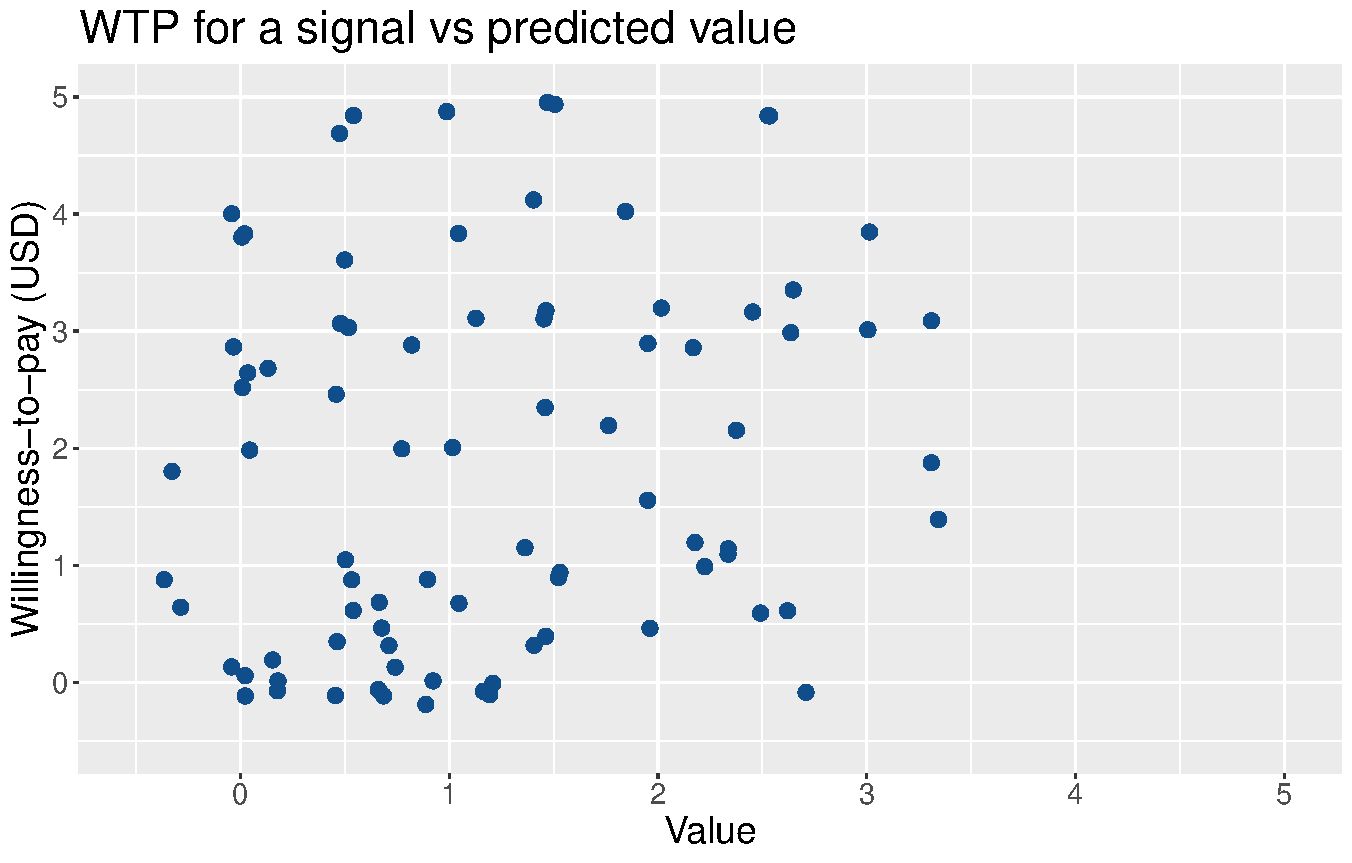
\includegraphics[scale=0.45]{Graphs/WTP_curve2.pdf}
\end{figure}
\end{frame}

\fi


\begin{frame}
\frametitle{Risk Aversion Measurement}
\begin{itemize}
\item Measure risk aversion based on blind protection choices:
\begin{itemize}
\item Exclude obs from subjects switching back and forth
\item The lowest probability for which a subject chooses to protect is $\pi^*$
\item Calculate their coefficient of relative risk aversion $\theta$ as the solution to the following equation:
$$\pi^* u(Y_0-L;\theta)+(1-\pi^*)u(Y_0;\theta)=u(Y_0-c;\theta)$$
\item Where  $u()$ is the CRRA utility function:
$$u(x;\theta)={x^{1-\theta} -1 \over 1-\theta}$$
\end{itemize}
\item Note: risk lovers have $\theta<0$
\end{itemize}
\end{frame}


\begin{frame}
\frametitle{Abnormal Protection Responses}
\begin{itemize}
\item Roughly one third of subjects (33 in the sample) switch from protection to no protection at least once
\item But only 6\% (6 subjects) switch more than once!
\item If a switcher becomes non-switcher after a single change, calculate the risk aversion based on the total number of switches
\item Left with only 7 subjects where this approach doesn't work and no risk aversion measurement is possible
\end{itemize}
\end{frame}


\begin{frame}
\frametitle{CRRA Estimates}
\begin{itemize}
\item Most subjects are moderately risk averse: 
\end{itemize}
\begin{table}[htbp]\centering

\begin{tabular}{l c c}
\hline\hline
Probability ($\pi^*$) &                $\theta$ & $N$\\
\hline
Always protect & $>$2 &   1 \\
0.1 & 2 & 10 \\
0.15 & 1.216 & 13 \\
0.2 & 0.573 & 29 \\
0.25 & 0 & 16 \\
0.3 & -0.539 & 15 \\
Never protect & $<$-0.539 &  14 \\
\hline
\end{tabular}
\end{table}
\end{frame}


\begin{frame}
\frametitle{WTP for the Signal}
\begin{itemize}
\item Theoretical value of the signal for risk-neutral subject:
$$b^*=\underbrace{\min[\pi L,c]}_{\text{BP costs}}-\underbrace{\pi(1-P(s=0|\omega=1))L}_{\text{False neg. costs}}-\underbrace{P(s=1)c}_{\text{Protection costs}}$$
\item Two potential approaches:
\begin{enumerate}
\item Regress the discrepancy between WTP $V$ and theoretical value $b^*$:
$$V-b^*=\alpha_0+\alpha_1\text{FN costs}+\alpha_2 \text{Prot. costs}+\epsilon$$
\item Regress WTP directly on its components and account for censoring at 0:
$$V=\min[0,\beta_0+\beta_1\text{FN costs}+\beta_2 \text{Prot. costs}-\beta_3\text{BP costs}+\gamma]$$
\item Note: protection costs include costs due to false positive signals
\end{enumerate}
\end{itemize}
\end{frame}


\begin{frame}
\frametitle{WTP Discrepancy Regressions}
\Large
\begin{itemize}
\item Regressing the difference between WTP and theoretical value for a risk-neutral subject
\item Coefficients should be zero
\end{itemize}
\normalsize
\end{frame}





\begin{frame}
\frametitle{WTP Discrepancy 1}

\footnotesize
\begin{table}[htbp]\centering
\def\sym#1{\ifmmode^{#1}\else\(^{#1}\)\fi}
\caption{WTP for Information (Discrepancy)}
\begin{tabular}{l*{4}{c}}
\hline\hline
                &\multicolumn{1}{c}{(1)}&\multicolumn{1}{c}{(2)}&\multicolumn{1}{c}{(3)}&\multicolumn{1}{c}{(4)}\\
                &\multicolumn{1}{c}{All}&\multicolumn{1}{c}{Risk-averse}&\multicolumn{1}{c}{Risk-loving}&\multicolumn{1}{c}{Switchers}\\
\hline
Prot. costs     &     .205\sym{**} &     .372\sym{**} &   -.0232         &     .183         \\
                &    (2.1)         &    (2.4)         &   (-0.1)         &    (1.0)         \\
False neg. costs&      .36\sym{***}&     .259\sym{**} &     .519\sym{***}&     .341\sym{**} \\
                &    (4.4)         &    (2.0)         &    (3.1)         &    (2.6)         \\
Constant        &    -.543\sym{***}&     -.58\sym{*}  &     -.54         &    -.441         \\
                &   (-2.8)         &   (-1.9)         &   (-1.5)         &   (-1.2)         \\
\hline
Observations    &      390         &      156         &      126         &      108         \\
Adjusted \(R^{2}\)&     0.05         &     0.05         &     0.07         &     0.04         \\
\hline\hline
\multicolumn{5}{l}{\footnotesize \textit{t} statistics in parentheses}\\
\multicolumn{5}{l}{\footnotesize \sym{*} \(p<0.10\), \sym{**} \(p<0.05\), \sym{***} \(p<0.01\)}\\
\end{tabular}
\end{table}

\normalsize
\end{frame}


\begin{frame}
\frametitle{WTP Discrepancy 2}
\begin{itemize}
\item Controlling for the prior probability of a black ball with dummies
\end{itemize}
\footnotesize
\begin{table}[htbp]\centering
\def\sym#1{\ifmmode^{#1}\else\(^{#1}\)\fi}
\caption{WTP for Information (Discrepancy)}
\begin{tabular}{l*{4}{c}}
\hline\hline
                &\multicolumn{1}{c}{(1)}&\multicolumn{1}{c}{(2)}&\multicolumn{1}{c}{(3)}&\multicolumn{1}{c}{(4)}\\
                &\multicolumn{1}{c}{All}&\multicolumn{1}{c}{Risk-averse}&\multicolumn{1}{c}{Risk-loving}&\multicolumn{1}{c}{Switchers}\\
\hline
False pos. costs&     .213\sym{**} &     .292\sym{**} &    .0744         &     .125         \\
                &    (2.3)         &    (2.3)         &    (0.5)         &    (0.3)         \\
False neg. costs&     .246\sym{***}&     .188\sym{**} &     .314\sym{***}&     .216         \\
                &    (4.2)         &    (2.3)         &    (3.4)         &    (1.0)         \\
Constant        &     .413\sym{***}&     .232         &     .463\sym{***}&     1.51\sym{**} \\
                &    (3.4)         &    (1.3)         &    (2.6)         &    (2.3)         \\
\hline
N obs.          &      744         &      336         &      354         &       54         \\
AIC             &     2673         &     1169         &     1296         &      212         \\
p(coeffs=0)     & .0000248\sym{***}&   .00525\sym{***}&   .00367\sym{***}&     .576         \\
\hline\hline
\multicolumn{5}{l}{\footnotesize \textit{t} statistics in parentheses}\\
\multicolumn{5}{l}{\footnotesize \sym{*} \(p<0.10\), \sym{**} \(p<0.05\), \sym{***} \(p<0.01\)}\\
\end{tabular}
\end{table}

\normalsize
\end{frame}





\begin{frame}
\frametitle{WTP Discrepancy 3 (Beliefs Accuracy)}
\footnotesize
\begin{table}[htbp]\centering
\def\sym#1{\ifmmode^{#1}\else\(^{#1}\)\fi}
\caption{WTP for Information (Discrepancy)}
\begin{tabular}{l*{3}{c}}
\hline\hline
                &\multicolumn{1}{c}{(1)}&\multicolumn{1}{c}{(2)}&\multicolumn{1}{c}{(3)}\\
                &\multicolumn{1}{c}{All}&\multicolumn{1}{c}{Accur. beliefs}&\multicolumn{1}{c}{Inaccur. beliefs}\\
\hline
False pos. costs&      .17         &   -.0437         &     .338\sym{**} \\
                &    (1.6)         &   (-0.3)         &    (2.3)         \\
False neg. costs&       .3\sym{***}&     .234\sym{***}&     .367\sym{***}\\
                &    (4.8)         &    (2.9)         &    (4.0)         \\
Constant        &    -.111         &   -.0405         &    -.173         \\
                &   (-1.2)         &   (-0.3)         &   (-1.2)         \\
\hline
N obs.          &      744         &      372         &      372         \\
AIC             &     2814         &     1389         &     1425         \\
p(coeffs=0)     & 5.45e-06\sym{***}&    .0153\sym{**} & .0000787\sym{***}\\
\hline\hline
\multicolumn{4}{l}{\footnotesize \textit{t} statistics in parentheses}\\
\multicolumn{4}{l}{\footnotesize \sym{*} \(p<0.10\), \sym{**} \(p<0.05\), \sym{***} \(p<0.01\)}\\
\end{tabular}
\end{table}

\normalsize
\end{frame}





\begin{frame}
\frametitle{WTP Discrepancy 4}
\begin{itemize}
\item Positive signal costs include costs of responding to true positive signal and the costs of responding to false positive signals
\end{itemize}
\footnotesize
\begin{table}[htbp]\centering
\def\sym#1{\ifmmode^{#1}\else\(^{#1}\)\fi}
\caption{WTP for Information (Discrepancy)}
\begin{tabular}{l*{4}{c}}
\hline\hline
                &\multicolumn{1}{c}{(1)}&\multicolumn{1}{c}{(2)}&\multicolumn{1}{c}{(3)}&\multicolumn{1}{c}{(4)}\\
                &\multicolumn{1}{c}{All}&\multicolumn{1}{c}{Risk-averse}&\multicolumn{1}{c}{Risk-loving}&\multicolumn{1}{c}{Switchers}\\
\hline
Pos. signal costs&     .191\sym{***}&     .335\sym{***}&    .0629         &   -.0304         \\
                &    (2.6)         &    (3.3)         &    (0.6)         &   (-0.1)         \\
False neg. costs&     .291\sym{***}&     .276\sym{***}&     .325\sym{***}&     .135         \\
                &    (4.7)         &    (3.2)         &    (3.3)         &    (0.7)         \\
Constant        &    -.342\sym{**} &      -.6\sym{***}&     -.21         &     .562         \\
                &   (-2.4)         &   (-3.0)         &   (-1.0)         &    (0.9)         \\
\hline
N obs.          &      744         &      336         &      354         &       54         \\
AIC             &     2810         &     1235         &     1361         &      215         \\
p(coeffs=0)     & 7.97e-07\sym{***}&  .000017\sym{***}&   .00419\sym{***}&     .772         \\
\hline\hline
\multicolumn{5}{l}{\footnotesize \textit{t} statistics in parentheses}\\
\multicolumn{5}{l}{\footnotesize \sym{*} \(p<0.10\), \sym{**} \(p<0.05\), \sym{***} \(p<0.01\)}\\
\end{tabular}
\end{table}

\normalsize
\end{frame}



\begin{frame}
\frametitle{WTP Discrepancy 5 (by Risk Aversion)}
\begin{itemize}
\item Explaining the discrepancy between WTP and value with risk aversion:
\end{itemize}
\footnotesize
\begin{table}[htbp]\centering
\def\sym#1{\ifmmode^{#1}\else\(^{#1}\)\fi}
\caption{WTP for Information (different risk aversion)}
\begin{tabular}{l*{6}{c}}
\hline\hline
                &\multicolumn{1}{c}{(1)}&\multicolumn{1}{c}{(2)}&\multicolumn{1}{c}{(3)}&\multicolumn{1}{c}{(4)}&\multicolumn{1}{c}{(5)}&\multicolumn{1}{c}{(6)}\\
                &\multicolumn{1}{c}{$\theta=0$}&\multicolumn{1}{c}{$\theta=0.5$}&\multicolumn{1}{c}{$\theta=1.0$}&\multicolumn{1}{c}{$\theta=1.5$}&\multicolumn{1}{c}{$\theta=2.5$}&\multicolumn{1}{c}{Heterogeneous $\theta$}\\
\hline
FP costs        &     .183         &     .212         &      .21         &     .165         &    .0499         &     .162         \\
                &    (0.1)         &    (0.1)         &    (0.1)         &    (0.1)         &    (0.1)         &    (0.1)         \\
FN costs        &     .212\sym{***}&     .317\sym{***}&     .431\sym{***}&      .53\sym{***}&      .66\sym{***}&     .234\sym{***}\\
                &    (0.1)         &    (0.1)         &    (0.1)         &    (0.1)         &    (0.1)         &    (0.1)         \\
Constant        &     .402\sym{**} &   .00285         &    -.516\sym{***}&    -1.17\sym{***}&    -1.67\sym{***}&   -.0609         \\
                &    (0.2)         &    (0.2)         &    (0.2)         &    (0.2)         &    (0.2)         &    (0.2)         \\
Prior dummies   &      Yes         &      Yes         &      Yes         &      Yes         &      Yes         &      Yes         \\
\hline
Observations    &      594         &      594         &      594         &      594         &      594         &      594         \\
Adjusted \(R^{2}\)&     0.19         &     0.24         &     0.25         &     0.30         &     0.35         &     0.12         \\
\hline\hline
\multicolumn{7}{l}{\footnotesize Standard errors in parentheses}\\
\multicolumn{7}{l}{\footnotesize \sym{*} \(p<0.10\), \sym{**} \(p<0.05\), \sym{***} \(p<0.01\)}\\
\end{tabular}
\end{table}

\end{frame}

\begin{frame}
\frametitle{Tobit Regressions}
\Large
\begin{itemize}
\item Regressing the WTP on its theoretical components
\item Censoring at 0 and at 5 USD
\item Coefficients should be one in absolute value
\item No constant in regressions
\end{itemize}
\normalsize
\end{frame}


\begin{frame}
\frametitle{WTP Tobit 1}

\footnotesize
\begin{table}[htbp]\centering
\def\sym#1{\ifmmode^{#1}\else\(^{#1}\)\fi}
\caption{WTP for Information (Tobit Estimation)}
\begin{tabular}{l*{4}{c}}
\hline\hline
                &\multicolumn{1}{c}{(1)}&\multicolumn{1}{c}{(2)}&\multicolumn{1}{c}{(3)}&\multicolumn{1}{c}{(4)}\\
                &\multicolumn{1}{c}{All}&\multicolumn{1}{c}{Risk-averse}&\multicolumn{1}{c}{Risk-loving}&\multicolumn{1}{c}{Switchers}\\
\hline
model           &                  &                  &                  &                  \\
BP costs        &     .541\sym{***}&     .549\sym{***}&     .537\sym{***}&     .386         \\
                &    (6.2)         &    (4.6)         &    (4.0)         &    (1.1)         \\
Prot. costs     &    -.274\sym{**} &    -.292         &    -.186         &     -.78         \\
                &   (-2.1)         &   (-1.6)         &   (-1.0)         &   (-1.4)         \\
False neg. costs&    -.471\sym{***}&     -.59\sym{***}&    -.357\sym{***}&    -.564         \\
                &   (-5.1)         &   (-4.3)         &   (-2.7)         &   (-1.5)         \\
Constant        &     .332         &     .325         &     .189         &     2.04         \\
                &    (1.2)         &    (0.8)         &    (0.5)         &    (1.5)         \\
\hline
sigma           &                  &                  &                  &                  \\
Constant        &     1.97\sym{***}&     1.91\sym{***}&     1.97\sym{***}&     2.18\sym{***}\\
                &   (28.0)         &   (18.7)         &   (19.6)         &    (7.0)         \\
\hline
Observations    &      630         &      288         &      300         &       42         \\
\textit{AIC}    &  2303.98         &  1038.72         &  1114.55         &   164.51         \\
\hline\hline
\multicolumn{5}{l}{\footnotesize \textit{t} statistics in parentheses}\\
\multicolumn{5}{l}{\footnotesize \sym{*} \(p<0.10\), \sym{**} \(p<0.05\), \sym{***} \(p<0.01\)}\\
\end{tabular}
\end{table}

\normalsize
\end{frame}


\begin{frame}
\frametitle{WTP Tobit 2: Splitting Protection Costs}

\footnotesize
\begin{table}[htbp]\centering
\def\sym#1{\ifmmode^{#1}\else\(^{#1}\)\fi}
\caption{WTP for Information (Tobit Estimation)}
\begin{tabular}{l*{4}{c}}
\hline\hline
                &\multicolumn{1}{c}{(1)}&\multicolumn{1}{c}{(2)}&\multicolumn{1}{c}{(3)}&\multicolumn{1}{c}{(4)}\\
                &\multicolumn{1}{c}{All}&\multicolumn{1}{c}{Risk-averse}&\multicolumn{1}{c}{Risk-loving}&\multicolumn{1}{c}{Switchers}\\
\hline
model           &                  &                  &                  &                  \\
BP costs        &     .688\sym{***}&     .635\sym{***}&     .704\sym{***}&      .74\sym{***}\\
                &   (12.0)         &    (6.3)         &    (7.2)         &    (7.5)         \\
Pos. signal costs&    -.373\sym{***}&    -.326         &    -.492\sym{**} &    -.329         \\
                &   (-3.0)         &   (-1.5)         &   (-2.3)         &   (-1.6)         \\
False neg. costs&    -.587\sym{***}&    -.619\sym{***}&    -.534\sym{***}&    -.625\sym{***}\\
                &   (-6.7)         &   (-3.9)         &   (-3.4)         &   (-4.6)         \\
\hline
N obs.          &      744         &      240         &      276         &      228         \\
AIC             &     2726         &      868         &     1026         &      841         \\
p(coeff=1)      & 6.68e-09\sym{***}&    .0028\sym{***}&   .00569\sym{***}& .0000643\sym{***}\\
\hline\hline
\multicolumn{5}{l}{\footnotesize \textit{t} statistics in parentheses}\\
\multicolumn{5}{l}{\footnotesize \sym{*} \(p<0.10\), \sym{**} \(p<0.05\), \sym{***} \(p<0.01\)}\\
\end{tabular}
\end{table}

\normalsize
\end{frame}


\begin{frame}
\frametitle{WTP Tobit 3: Controlling for Prior Probability}

\footnotesize
\begin{table}[htbp]\centering
\def\sym#1{\ifmmode^{#1}\else\(^{#1}\)\fi}
\caption{WTP Tobit (Prob Dummies)}
\begin{tabular}{l*{4}{c}}
\hline\hline
                &\multicolumn{1}{c}{(1)}&\multicolumn{1}{c}{(2)}&\multicolumn{1}{c}{(3)}&\multicolumn{1}{c}{(4)}\\
                &\multicolumn{1}{c}{All}&\multicolumn{1}{c}{Risk-averse}&\multicolumn{1}{c}{Risk-loving}&\multicolumn{1}{c}{Switchers}\\
\hline
model           &                  &                  &                  &                  \\
False pos. costs&    -.332\sym{**} &    -.324\sym{*}  &    -.456\sym{*}  &     .154         \\
                &   (-2.3)         &   (-1.7)         &   (-2.0)         &    (0.3)         \\
False neg. costs&    -.505\sym{***}&    -.547\sym{***}&    -.448\sym{***}&     -.52         \\
                &   (-5.3)         &   (-4.3)         &   (-3.0)         &   (-1.4)         \\
\hline
N obs.          &      744         &      336         &      354         &       54         \\
AIC             &     2775         &     1220         &     1342         &      223         \\
p(coeff=1)      & 3.08e-12\sym{***}& 4.15e-07\sym{***}& .0000457\sym{***}&    .0693\sym{*}  \\
\hline\hline
\multicolumn{5}{l}{\footnotesize \textit{t} statistics in parentheses}\\
\multicolumn{5}{l}{\footnotesize \sym{*} \(p<0.10\), \sym{**} \(p<0.05\), \sym{***} \(p<0.01\)}\\
\end{tabular}
\end{table}

\normalsize
\end{frame}


\iffalse
\begin{frame}
\frametitle{WTP Tobit 3 (Conservative Classification)}
\begin{itemize}
\item Any crossing from protection to no protection=switcher
\end{itemize}
\footnotesize
\begin{table}[htbp]\centering
\def\sym#1{\ifmmode^{#1}\else\(^{#1}\)\fi}
\caption{WTP for Information (Tobit Estimation)}
\begin{tabular}{l*{4}{c}}
\hline\hline
                &\multicolumn{1}{c}{(1)}&\multicolumn{1}{c}{(2)}&\multicolumn{1}{c}{(3)}&\multicolumn{1}{c}{(4)}\\
                &\multicolumn{1}{c}{All}&\multicolumn{1}{c}{Risk-averse}&\multicolumn{1}{c}{Risk-loving}&\multicolumn{1}{c}{Switchers}\\
\hline
model           &                  &                  &                  &                  \\
BP costs        &     .688\sym{***}&     .635\sym{***}&     .704\sym{***}&      .74\sym{***}\\
                &   (12.0)         &    (6.3)         &    (7.2)         &    (7.5)         \\
Pos. signal costs&    -.373\sym{***}&    -.326         &    -.492\sym{**} &    -.329         \\
                &   (-3.0)         &   (-1.5)         &   (-2.3)         &   (-1.6)         \\
False neg. costs&    -.587\sym{***}&    -.619\sym{***}&    -.534\sym{***}&    -.625\sym{***}\\
                &   (-6.7)         &   (-3.9)         &   (-3.4)         &   (-4.6)         \\
\hline
N obs.          &      744         &      240         &      276         &      228         \\
AIC             &     2726         &      868         &     1026         &      841         \\
p(coeff=1)      & 6.68e-09\sym{***}&    .0028\sym{***}&   .00569\sym{***}& .0000643\sym{***}\\
\hline\hline
\multicolumn{5}{l}{\footnotesize \textit{t} statistics in parentheses}\\
\multicolumn{5}{l}{\footnotesize \sym{*} \(p<0.10\), \sym{**} \(p<0.05\), \sym{***} \(p<0.01\)}\\
\end{tabular}
\end{table}

\normalsize
\end{frame}



\begin{frame}
\frametitle{WTP Tobit 3 (Belief Accuracy)}
\begin{itemize}
\item Accurate beliefs=total abs. belief elicitation error$<$median
\item Subject with accurate beliefs are more sensitive to signal characteristics (but diffs are insignificant at 5\%)
\end{itemize}
\footnotesize
\begin{table}[htbp]\centering
\def\sym#1{\ifmmode^{#1}\else\(^{#1}\)\fi}
\caption{WTP for Information (Tobit Estimation)}
\begin{tabular}{l*{3}{c}}
\hline\hline
                &\multicolumn{1}{c}{(1)}&\multicolumn{1}{c}{(2)}&\multicolumn{1}{c}{(3)}\\
                &\multicolumn{1}{c}{All}&\multicolumn{1}{c}{Accur. beliefs}&\multicolumn{1}{c}{Inaccur. beliefs}\\
\hline
model           &                  &                  &                  \\
BP costs        &     .688\sym{***}&      .77\sym{***}&     .613\sym{***}\\
                &   (12.0)         &    (9.7)         &    (7.4)         \\
Pos. signal costs&    -.373\sym{***}&    -.538\sym{***}&    -.224         \\
                &   (-3.0)         &   (-3.1)         &   (-1.3)         \\
False neg. costs&    -.587\sym{***}&    -.749\sym{***}&    -.422\sym{***}\\
                &   (-6.7)         &   (-6.2)         &   (-3.3)         \\
\hline
N obs.          &      744         &      372         &      372         \\
AIC             &     2726         &     1356         &     1372         \\
p(coeff=1)      & 6.68e-09\sym{***}&    .0202\sym{**} & 1.44e-07\sym{***}\\
\hline\hline
\multicolumn{4}{l}{\footnotesize \textit{t} statistics in parentheses}\\
\multicolumn{4}{l}{\footnotesize \sym{*} \(p<0.10\), \sym{**} \(p<0.05\), \sym{***} \(p<0.01\)}\\
\end{tabular}
\end{table}

\normalsize
\end{frame}



\begin{frame}
\frametitle{Risk-averse vs Risk-loving}
\begin{itemize}
\item Estimate Tobit models separately for risk-averse and risk-loving subjects (includes risk-neutral) 
\item Then use Wald tests on coefficients (no assumpt. of equal variance); alternative - bootstrap
\item Higher sensitivity to false negative rates for risk-averse subjects
\item The difference is not stat. significant (p=0.23)
\item The differences are even less significant for other coeffs
\item \textbf{Cannot reject the hypothesis that coeffs completely match in two models (p=0.58)}
\end{itemize}
\end{frame}


\begin{frame}
\frametitle{False-positive vs False-negative payoff}
\begin{itemize}
\item Test equality of coefficients on false-positive (-0.37) and false-negative costs (-0.59)
\begin{itemize}
\item Significance: $p=0.12$ (standard), $p=0.08$ (1000 bootstrap)
\end{itemize}
\item Linear regression has lower variances (so that respective $p=0.008$ and $p=0.023$)
\end{itemize}
\end{frame}
\fi



\begin{frame}
\frametitle{Actual Costs vs Theoretical Costs}
\begin{itemize}
\item Calculate actual costs based on decisions made in the Informed Protection treatment and actual posterior probabilities of losses.
\item Each reported participant's strategy $s$ is a tuple of numbers $(r_w,r_b)$ representing protection responses correspondingly to white and black hints
\item Then the expected cost of each decision are:
\small
$$EC(s)=\pi (P(0|1)(1-r_w)+P(1|1)(1-r_b))L+P(s=1)c$$
$$+(P(s=0)r_w+P(s=1)r_b)c$$
\normalsize
\item Regress expected costs on minimal theoretical costs and other signal characteristics
\end{itemize}
\end{frame}


\begin{frame}
\frametitle{Actual Costs vs Theoretical Costs}
\begin{itemize}
\item Prior prob and false negative rates disproportionally affect expected costs:
\end{itemize}
\footnotesize
\begin{table}[htbp]\centering
\def\sym#1{\ifmmode^{#1}\else\(^{#1}\)\fi}
\caption{Actual Exp. Costs vs Theoretical Costs}
\begin{tabular}{l*{6}{c}}
\hline\hline
                &\multicolumn{1}{c}{(1)}&\multicolumn{1}{c}{(2)}&\multicolumn{1}{c}{(3)}&\multicolumn{1}{c}{(4)}&\multicolumn{1}{c}{(5)}&\multicolumn{1}{c}{(6)}\\
                &\multicolumn{1}{c}{OLS}&\multicolumn{1}{c}{OLS}&\multicolumn{1}{c}{OLS}&\multicolumn{1}{c}{FE}&\multicolumn{1}{c}{FE}&\multicolumn{1}{c}{FE}\\
\hline
Optimal exp. costs&     1.04\sym{***}&     .842\sym{***}&     .592         &     1.04\sym{***}&     .879\sym{***}&     1.13\sym{***}\\
                &    (9.4)         &    (4.3)         &    (1.3)         &   (10.7)         &    (4.1)         &    (9.3)         \\
Prior prob.     &                  &    -2.19         &    -3.69         &                  &    -2.07         &                  \\
                &                  &   (-1.1)         &   (-1.2)         &                  &   (-1.1)         &                  \\
False neg. rate &                  &                  &    -2.68         &                  &                  &    -.696         \\
                &                  &                  &   (-1.6)         &                  &                  &   (-0.6)         \\
False pos. rate &                  &                  &     .713         &                  &                  &     2.51         \\
                &                  &                  &    (0.4)         &                  &                  &    (1.4)         \\
Constant        &    -.888\sym{***}&    -.733\sym{**} &    -.662\sym{**} &    -.875\sym{***}&    -.684\sym{***}&    -.918\sym{***}\\
                &   (-3.3)         &   (-2.6)         &   (-2.2)         &   (-4.0)         &   (-3.3)         &   (-4.3)         \\
\hline
Observations    &      150         &      150         &      150         &      150         &      150         &      150         \\
Adjusted \(R^{2}\)&     0.34         &     0.35         &     0.36         &     0.41         &     0.42         &     0.43         \\
\hline\hline
\multicolumn{7}{l}{\footnotesize \textit{t} statistics in parentheses}\\
\multicolumn{7}{l}{\footnotesize \sym{*} \(p<0.10\), \sym{**} \(p<0.05\), \sym{***} \(p<0.01\)}\\
\end{tabular}
\end{table}

\end{frame}

\begin{frame}
\frametitle{Actual Costs - Theoretical Costs Discrepancy}
\begin{itemize}
\item Prior prob and false negative rates disproportionally affect expected costs:
\end{itemize}
\footnotesize
\begin{table}[htbp]\centering
\def\sym#1{\ifmmode^{#1}\else\(^{#1}\)\fi}
\caption{Expected costs discrepancy}
\begin{tabular}{l*{6}{c}}
\hline\hline
                &\multicolumn{1}{c}{(1)}&\multicolumn{1}{c}{(2)}&\multicolumn{1}{c}{(3)}&\multicolumn{1}{c}{(4)}&\multicolumn{1}{c}{(5)}&\multicolumn{1}{c}{(6)}\\
                &\multicolumn{1}{c}{}&\multicolumn{1}{c}{}&\multicolumn{1}{c}{}&\multicolumn{1}{c}{}&\multicolumn{1}{c}{}&\multicolumn{1}{c}{}\\
\hline
FP costs        &    .0438         &    .0142         &    .0512         &    .0505         &    .0318         &   -.0582         \\
                &    (0.4)         &    (0.1)         &    (0.4)         &    (0.3)         &    (0.2)         &   (-0.4)         \\
FN costs        &   -.0137         &    .0227         &    -.132         &     -.13         &     .163\sym{**} &     .287\sym{**} \\
                &   (-0.2)         &    (0.3)         &   (-1.4)         &   (-1.1)         &    (2.0)         &    (2.5)         \\
Risk-averse     &                  &                  &    -.284         &    .0641         &                  &                  \\
                &                  &                  &   (-1.4)         &    (0.3)         &                  &                  \\
Risk-averse $\times$ FP costs&                  &                  &   -.0282         &   -.0629         &                  &                  \\
                &                  &                  &   (-0.1)         &   (-0.3)         &                  &                  \\
Risk-averse $\times$ FN costs&                  &                  &      .22\sym{*}  &     .269\sym{*}  &                  &                  \\
                &                  &                  &    (1.9)         &    (1.7)         &                  &                  \\
Accur. beliefs  &                  &                  &                  &                  &     .613\sym{***}&    .0902         \\
                &                  &                  &                  &                  &    (3.2)         &    (0.4)         \\
Accur. beliefs $\times$ FP costs&                  &                  &                  &                  &    .0566         &     .185         \\
                &                  &                  &                  &                  &    (0.3)         &    (1.0)         \\
Accur. beliefs $\times$ FN costs&                  &                  &                  &                  &    -.354\sym{***}&    -.522\sym{***}\\
                &                  &                  &                  &                  &   (-3.0)         &   (-3.5)         \\
Constant        &    -.857\sym{***}&    -.706\sym{***}&    -.684\sym{***}&    -.754\sym{***}&    -1.17\sym{***}&    -.758\sym{***}\\
                &   (-8.9)         &   (-6.4)         &   (-5.4)         &   (-4.7)         &   (-7.7)         &   (-5.1)         \\
Prior prob dummies &       No         &      Yes         &       No         &      Yes         &       No         &      Yes         \\
\hline
Observations    &      743         &      743         &      689         &      689         &      743         &      743         \\
Adjusted \(R^{2}\)&    -0.00         &    -0.00         &    -0.00         &    -0.00         &     0.02         &     0.04         \\
\hline\hline
\multicolumn{7}{l}{\footnotesize \textit{t} statistics in parentheses}\\
\multicolumn{7}{l}{\footnotesize \sym{*} \(p<0.10\), \sym{**} \(p<0.05\), \sym{***} \(p<0.01\)}\\
\end{tabular}
\end{table}

\end{frame}


\begin{frame}
\frametitle{Actual Costs - Theoretical Costs Discrepancy 2}
\begin{itemize}
\item Prior prob and false negative rates disproportionally affect expected costs:
\end{itemize}
\footnotesize
\begin{table}[htbp]\centering
\def\sym#1{\ifmmode^{#1}\else\(^{#1}\)\fi}
\caption{Expected costs discrepancy (without 10\% outliers)}
\begin{tabular}{l*{6}{c}}
\hline\hline
                &\multicolumn{1}{c}{(1)}&\multicolumn{1}{c}{(2)}&\multicolumn{1}{c}{(3)}&\multicolumn{1}{c}{(4)}&\multicolumn{1}{c}{(5)}&\multicolumn{1}{c}{(6)}\\
                &\multicolumn{1}{c}{}&\multicolumn{1}{c}{}&\multicolumn{1}{c}{}&\multicolumn{1}{c}{}&\multicolumn{1}{c}{}&\multicolumn{1}{c}{}\\
\hline
FP costs        &    -.229\sym{***}&    -.208\sym{***}&    -.145\sym{**} &    -.122\sym{*}  &     -.27\sym{***}&    -.113\sym{*}  \\
                &   (-4.2)         &   (-4.0)         &   (-2.1)         &   (-1.9)         &   (-3.2)         &   (-1.7)         \\
FN costs        &     -.12\sym{***}&     -.13\sym{***}&    -.138\sym{***}&    -.154\sym{***}&   -.0714\sym{*}  &    -.145\sym{***}\\
                &   (-4.2)         &   (-4.1)         &   (-3.5)         &   (-3.8)         &   (-1.7)         &   (-3.8)         \\
Risk-averse     &                  &                  &    -.135\sym{*}  &   -.0101         &                  &    -.122\sym{*}  \\
                &                  &                  &   (-1.9)         &   (-0.1)         &                  &   (-1.7)         \\
Risk-averse $\times$ FP costs&                  &                  &    -.116         &    -.103         &                  &    -.101         \\
                &                  &                  &   (-1.0)         &   (-1.0)         &                  &   (-0.9)         \\
Risk-averse $\times$ FN costs&                  &                  &    .0319         &    .0286         &                  &    .0157         \\
                &                  &                  &    (0.5)         &    (0.4)         &                  &    (0.3)         \\
Accur. beliefs  &                  &                  &                  &                  &     .182\sym{***}&     .214\sym{***}\\
                &                  &                  &                  &                  &    (2.7)         &    (3.1)         \\
Accur. beliefs $\times$ FP costs&                  &                  &                  &                  &     .102         &                  \\
                &                  &                  &                  &                  &    (1.0)         &                  \\
Accur. beliefs $\times$ FN costs&                  &                  &                  &                  &   -.0933         &                  \\
                &                  &                  &                  &                  &   (-1.6)         &                  \\
Constant        &    -.185\sym{***}&   -.0718         &    -.133\sym{***}&   -.0814         &    -.283\sym{***}&    -.137\sym{*}  \\
                &   (-5.6)         &   (-1.6)         &   (-3.5)         &   (-1.4)         &   (-5.0)         &   (-1.9)         \\
Prior prob dummies &       No         &      Yes         &       No         &      Yes         &       No         &      Yes         \\
\hline
Observations    &      658         &      658         &      614         &      614         &      658         &      614         \\
Adjusted \(R^{2}\)&     0.05         &     0.07         &     0.06         &     0.09         &     0.06         &     0.11         \\
\hline\hline
\multicolumn{7}{l}{\footnotesize \textit{t} statistics in parentheses}\\
\multicolumn{7}{l}{\footnotesize \sym{*} \(p<0.10\), \sym{**} \(p<0.05\), \sym{***} \(p<0.01\)}\\
\end{tabular}
\end{table}

\end{frame}



\begin{frame}
\frametitle{Value Formation}
\begin{itemize}
\item What drives the difference between theoretical value and actual willingness-to-pay? Potential elements affecting the WTP:
\begin{itemize}
\item Beliefs
\item Strategies
\item Preferences
\end{itemize}
\item We recalculate the value after incorporating these elements one-by-one
\end{itemize}
%\footnotesize
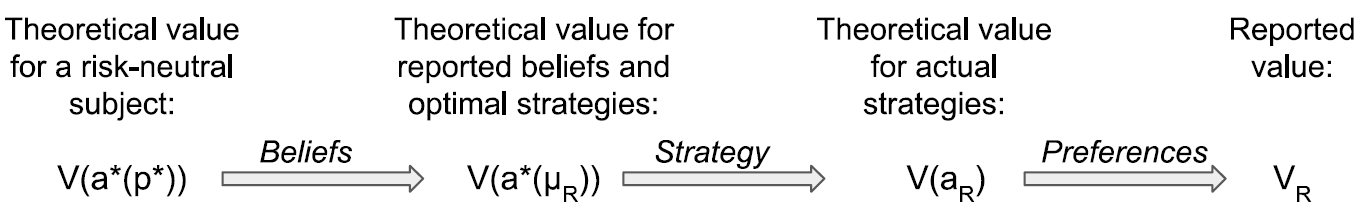
\includegraphics[scale=0.4]{value_diagram.png}
\end{frame}


\begin{frame}
\frametitle{Value Formation}
\begin{itemize}
\item Accounting for reported beliefs or strategies does not make the theoretical value closer to the WTP
\item WTP is still more correlated with the (completely) theoretical value rather than with values accounting for beliefs $\mu_R$ or strategies $a_R$
\item My hypothesis: subjects approach the tasks independently and/or do not report beliefs truthfully
\end{itemize}

\begin{table}[htbp]\centering

\begin{tabular}{l c c c c}
\hline\hline
           & $V(a^*(p^*))$ & $V(a^*(\mu_R))$   & $V(a_R)$ & $V_R$\\
\hline
$V(a^*(p^*))$ & 1 &   0.52 & 0.54 & 0.34\\
$V(a^*(\mu_R))$ & 0.52 & 1 & 0.63 & 0.29  \\
$V(a_R)$ & 0.54 & 0.63 & 1 & 0.33\\
$V_R$ & 0.34 & 0.29 & 0.33 & 1 \\

\hline
\end{tabular}
\end{table}

\end{frame}



\begin{frame}
\frametitle{Additional Complementary Tables}
\begin{enumerate}
\item Belief updating (slides are not updated)
\item Determinants of informed protection responses
\item Classifying informed protection strategies
\item Extra WTP tables
\end{enumerate}
\end{frame}


\iffalse
\begin{frame}
\frametitle{Belief Updating}
\begin{itemize}
\item A bit more correlation with actual posterior probabilities!
\item Even more if we exclude everybody scoring less than 7 out of 10 quiz questions
\end{itemize}
\begin{figure}[h]
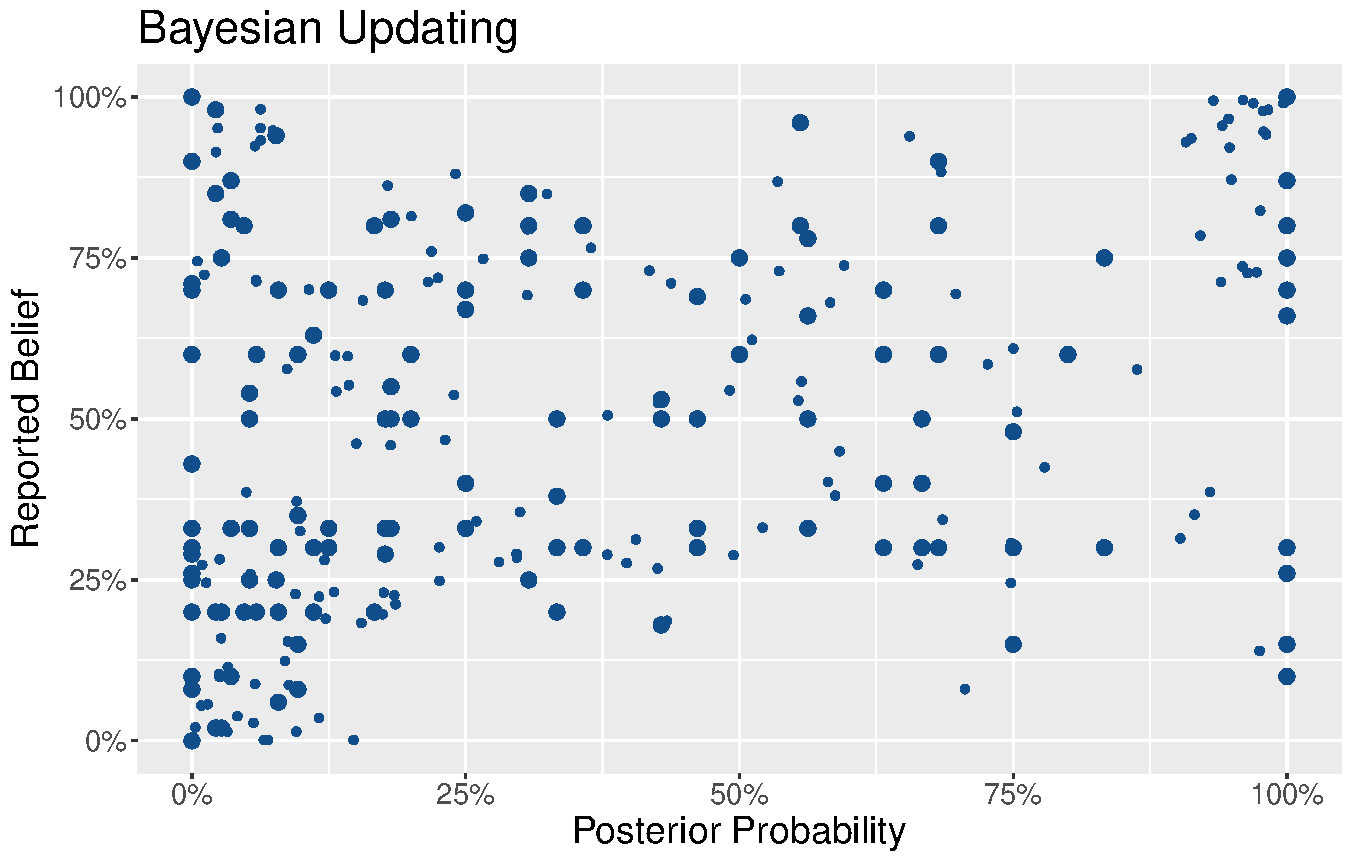
\includegraphics[scale=0.4]{Graphs/UPD_curve2.pdf}
\end{figure}
\end{frame}
\fi



\begin{frame}
\frametitle{Belief Updating: Correlation}
%\footnotesize
\begin{table}[htbp]\centering
\def\sym#1{\ifmmode^{#1}\else\(^{#1}\)\fi}
\caption{Belief Elicitation: Belief vs Posterior}
\begin{tabular}{l*{3}{c}}
\hline\hline
                &\multicolumn{1}{c}{(1)}&\multicolumn{1}{c}{(2)}&\multicolumn{1}{c}{(3)}\\
                &\multicolumn{1}{c}{All}&\multicolumn{1}{c}{Not\_honest}&\multicolumn{1}{c}{Good quiz}\\
\hline
Posterior prob. &     .669\sym{***}&     .711\sym{***}&     .523\sym{***}\\
                &   (29.0)         &   (29.1)         &   (15.7)         \\
Constant        &     .151\sym{***}&     .147\sym{***}&     .226\sym{***}\\
                &   (16.2)         &   (14.1)         &   (17.8)         \\
\hline
Observations    &      780         &      636         &      520         \\
Adjusted \(R^{2}\)&     0.57         &     0.61         &     0.39         \\
\hline\hline
\multicolumn{4}{l}{\footnotesize \textit{t} statistics in parentheses}\\
\multicolumn{4}{l}{\footnotesize \sym{*} \(p<0.10\), \sym{**} \(p<0.05\), \sym{***} \(p<0.01\)}\\
\end{tabular}
\end{table}


\end{frame}

\begin{frame}
\frametitle{Belief Updating: Decomposition}
\begin{itemize}
\item Posterior probability $\mu=P(B|S=x)$ that the ball is black conditional on a hint $S=x$ can be written as:
$$\ln \left({\mu \over 1-\mu} \right)=\lambda_0+S_B+S_W$$
\item With $\lambda_0\equiv \ln(p/(1-p))$ representing (transformed) prior beliefs
\item And $S_B$, $S_W$ describing the effect of new evidence:
$$S_B\equiv I(S=B)\ln(P(s=B|B)/P(s=B|W))$$
$$S_W\equiv I(S=W)\ln((1-P(s=B|B))/(1-P(s=B|W))$$
\end{itemize}
\end{frame}


\begin{frame}
\frametitle{Belief Updating: Decomposition}
%\footnotesize
\begin{table}[htbp]\centering
\def\sym#1{\ifmmode^{#1}\else\(^{#1}\)\fi}
\caption{Belief Elicitation: Decomposition}
\begin{tabular}{l*{3}{c}}
\hline\hline
                &\multicolumn{1}{c}{(1)}&\multicolumn{1}{c}{(2)}&\multicolumn{1}{c}{(3)}\\
                &\multicolumn{1}{c}{OLS}&\multicolumn{1}{c}{FE}&\multicolumn{1}{c}{Smart, FE}\\
\hline
lt\_prior        &     .178         &     .205\sym{**} &     .231\sym{**} \\
                &    (1.4)         &    (2.5)         &    (2.2)         \\
signalB         &   -.0835         &     .735\sym{**} &     .988\sym{**} \\
                &   (-0.2)         &    (2.5)         &    (2.5)         \\
signalW         &     .818\sym{***}&        0         &        0         \\
                &    (2.8)         &      (.)         &      (.)         \\
Constant        &     .332         &    -.471\sym{**} &    -.577\sym{**} \\
                &    (0.9)         &   (-2.7)         &   (-2.6)         \\
\hline
Observations    &       68         &       68         &       52         \\
Adjusted \(R^{2}\)&     0.16         &     0.20         &     0.25         \\
\hline\hline
\multicolumn{4}{l}{\footnotesize \textit{t} statistics in parentheses}\\
\multicolumn{4}{l}{\footnotesize \sym{*} \(p<0.10\), \sym{**} \(p<0.05\), \sym{***} \(p<0.01\)}\\
\end{tabular}
\end{table}

\end{frame}



\begin{frame}
\frametitle{Informed Protection: Determinants}
\footnotesize
\begin{table}[htbp]\centering
\def\sym#1{\ifmmode^{#1}\else\(^{#1}\)\fi}
\caption{Informed Protection}
\begin{tabular}{l*{4}{c}}
\hline\hline
                &\multicolumn{1}{c}{(1)}&\multicolumn{1}{c}{(2)}&\multicolumn{1}{c}{(3)}&\multicolumn{1}{c}{(4)}\\
                &\multicolumn{1}{c}{All}&\multicolumn{1}{c}{All}&\multicolumn{1}{c}{Smart}&\multicolumn{1}{c}{Smart}\\
\hline
Posterior prob. &     .663\sym{***}&     .114         &     .692\sym{***}&     .126         \\
                &    (8.5)         &    (0.9)         &    (9.4)         &    (0.8)         \\
Prior prob.     &                  &     .467\sym{***}&                  &     .519\sym{***}\\
                &                  &    (3.5)         &                  &    (3.1)         \\
Gremlin says Black&                  &     .497\sym{***}&                  &     .506\sym{***}\\
                &                  &    (5.8)         &                  &    (5.0)         \\
Constant        &     .235\sym{***}&    .0872\sym{**} &     .233\sym{***}&    .0678         \\
                &    (7.3)         &    (2.2)         &    (7.7)         &    (1.6)         \\
\hline
Observations    &      300         &      300         &      228         &      228         \\
Adjusted \(R^{2}\)&     0.35         &     0.41         &     0.36         &     0.42         \\
\hline\hline
\multicolumn{5}{l}{\footnotesize \textit{t} statistics in parentheses}\\
\multicolumn{5}{l}{\footnotesize \sym{*} \(p<0.10\), \sym{**} \(p<0.05\), \sym{***} \(p<0.01\)}\\
\end{tabular}
\end{table}


\end{frame}


\begin{frame}
\frametitle{Informed Protection: Reacting to Own Beliefs or Posterior Probabilties?}
%\footnotesize
\begin{table}[htbp]\centering
\def\sym#1{\ifmmode^{#1}\else\(^{#1}\)\fi}
\caption{Informed Protection: Response to Reported Beliefs}
\begin{tabular}{l*{3}{c}}
\hline\hline
                &\multicolumn{1}{c}{(1)}&\multicolumn{1}{c}{(2)}&\multicolumn{1}{c}{(3)}\\
                &\multicolumn{1}{c}{All}&\multicolumn{1}{c}{All}&\multicolumn{1}{c}{Smart}\\
\hline
Belief          &     .746\sym{***}&     .358\sym{**} &     .462\sym{**} \\
                &    (7.8)         &    (2.4)         &    (2.5)         \\
Posterior prob. &                  &     .424\sym{***}&     .367\sym{**} \\
                &                  &    (3.5)         &    (2.6)         \\
Constant        &     .206\sym{***}&     .189\sym{***}&     .178\sym{***}\\
                &    (5.3)         &    (4.8)         &    (4.6)         \\
\hline
Observations    &      300         &      300         &      228         \\
Adjusted \(R^{2}\)&     0.32         &     0.38         &     0.40         \\
\hline\hline
\multicolumn{4}{l}{\footnotesize \textit{t} statistics in parentheses}\\
\multicolumn{4}{l}{\footnotesize \sym{*} \(p<0.10\), \sym{**} \(p<0.05\), \sym{***} \(p<0.01\)}\\
\end{tabular}
\end{table}

\end{frame}


\begin{frame}
\frametitle{Informed Protection: Do Subject's Beliefs Matter?}
%\footnotesize
\begin{table}[htbp]\centering
\def\sym#1{\ifmmode^{#1}\else\(^{#1}\)\fi}
\caption{Informed Protection: Response to Reported Beliefs}
\begin{tabular}{l*{4}{c}}
\hline\hline
                &\multicolumn{1}{c}{(1)}&\multicolumn{1}{c}{(2)}&\multicolumn{1}{c}{(3)}&\multicolumn{1}{c}{(4)}\\
                &\multicolumn{1}{c}{}&\multicolumn{1}{c}{}&\multicolumn{1}{c}{}&\multicolumn{1}{c}{}\\
\hline
Informed protection&                  &                  &                  &                  \\
Belief          &     2.36\sym{***}&     2.67\sym{***}&     2.63\sym{***}&     2.85\sym{***}\\
                &    (0.2)         &    (0.2)         &    (0.4)         &    (0.4)         \\
Belief error    &                  &      1.3\sym{***}&     1.17\sym{***}&     1.44\sym{***}\\
                &                  &    (0.2)         &    (0.2)         &    (0.3)         \\
Good quiz       &                  &                  &     .184         &                  \\
                &                  &                  &    (0.2)         &                  \\
Good quiz $\times$ Belief&                  &                  &     .105         &                  \\
                &                  &                  &    (0.5)         &                  \\
Good quiz $\times$ Belief error&                  &                  &      .34         &                  \\
                &                  &                  &    (0.4)         &                  \\
Stat. class     &                  &                  &                  &    .0954         \\
                &                  &                  &                  &    (0.2)         \\
Stat. class $\times$ Belief&                  &                  &                  &    -.287         \\
                &                  &                  &                  &    (0.5)         \\
Stat. class $\times$ Belief error&                  &                  &                  &    -.212         \\
                &                  &                  &                  &    (0.4)         \\
Constant        &    -.813\sym{***}&    -.914\sym{***}&    -1.01\sym{***}&    -.973\sym{***}\\
                &    (0.1)         &    (0.1)         &    (0.2)         &    (0.1)         \\
\hline
Observations    &     1259         &     1259         &     1259         &     1259         \\
\textit{AIC}    &  1287.47         &  1196.40         &  1194.29         &  1201.09         \\
\hline\hline
\multicolumn{5}{l}{\footnotesize Standard errors in parentheses}\\
\multicolumn{5}{l}{\footnotesize \sym{*} \(p<0.10\), \sym{**} \(p<0.05\), \sym{***} \(p<0.01\)}\\
\end{tabular}
\end{table}

\end{frame}


\begin{frame}
\frametitle{Informed Protection: Responding to Beliefs or Posterior Probabilities}
\begin{itemize}
\item Calculate the subject-specific correlation between beliefs, posterior probabilities and protection responses
\item Mann-Whitney U-test as  a correlation measure with two "groups": signals answered with either protection or no protection responses
\item No obvious clustering, but $\exists$ three groups:
\begin{enumerate}
\item Sophisticated: protection decisions closely follow their accurate beliefs
\item Clueless: protection decisions follow neither posteriors nor reported beliefs
\item Amenders: have inaccurate beliefs, but behave consistently with posterior probabilities (small group)
\end{enumerate}
\end{itemize}
\end{frame}



\begin{frame}
\frametitle{Informed Protection: Responding to Beliefs or Posterior Probabilities}

%\footnotesize
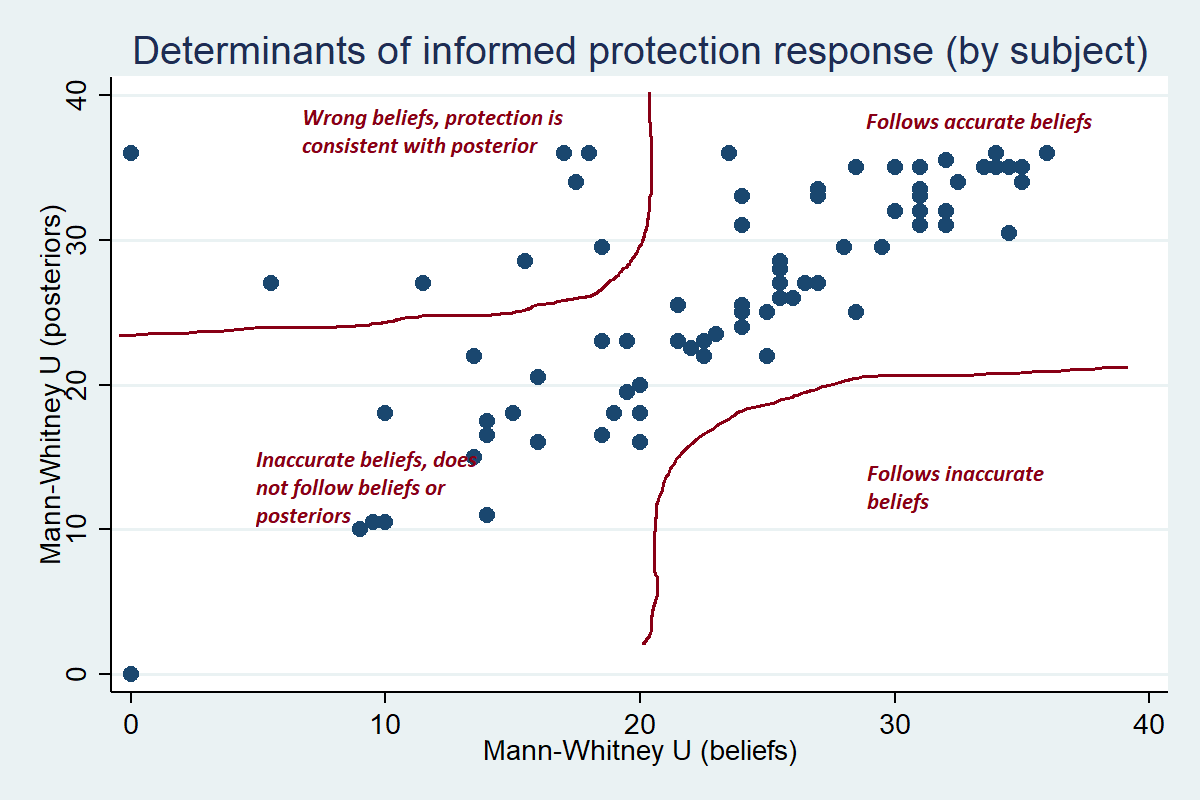
\includegraphics[scale=0.45]{Graphs/clustering1.png}
\end{frame}





\begin{frame}
\frametitle{WTP Discrepancy 6}
\begin{itemize}
\item Adding blind protection costs
\end{itemize}
\footnotesize
\begin{table}[htbp]\centering
\def\sym#1{\ifmmode^{#1}\else\(^{#1}\)\fi}
\caption{WTP for Information (Discrepancy)}
\begin{tabular}{l*{4}{c}}
\hline\hline
                &\multicolumn{1}{c}{(1)}&\multicolumn{1}{c}{(2)}&\multicolumn{1}{c}{(3)}&\multicolumn{1}{c}{(4)}\\
                &\multicolumn{1}{c}{All}&\multicolumn{1}{c}{Risk-averse}&\multicolumn{1}{c}{Risk-loving}&\multicolumn{1}{c}{Switchers}\\
\hline
BP costs        &    -.519\sym{***}&    -.484\sym{***}&    -.534\sym{***}&    -.622\sym{**} \\
                &   (-9.3)         &   (-6.2)         &   (-6.6)         &   (-2.5)         \\
Pos. signal costs&     .671\sym{***}&     .759\sym{***}&     .596\sym{***}&     .482         \\
                &    (8.0)         &    (6.8)         &    (4.5)         &    (1.4)         \\
False neg. costs&     .475\sym{***}&     .423\sym{***}&     .542\sym{***}&     .371\sym{*}  \\
                &    (7.3)         &    (4.6)         &    (5.2)         &    (1.7)         \\
Constant        &     .818\sym{***}&     .526\sym{**} &     .917\sym{***}&     2.06\sym{**} \\
                &    (4.6)         &    (2.1)         &    (3.6)         &    (2.5)         \\
\hline
N obs.          &      744         &      336         &      354         &       54         \\
AIC             &     2738         &     1206         &     1326         &      210         \\
p(coeffs=0)     & 3.83e-22\sym{***}& 2.00e-12\sym{***}& 8.46e-10\sym{***}&    .0958\sym{*}  \\
\hline\hline
\multicolumn{5}{l}{\footnotesize \textit{t} statistics in parentheses}\\
\multicolumn{5}{l}{\footnotesize \sym{*} \(p<0.10\), \sym{**} \(p<0.05\), \sym{***} \(p<0.01\)}\\
\end{tabular}
\end{table}

\normalsize
\end{frame}



\begin{frame}
\frametitle{WTP Discrepancy 7}
\begin{itemize}
\item Controlling for the prior probability of a black ball with dummies
\end{itemize}
\footnotesize
\begin{table}[htbp]\centering
\def\sym#1{\ifmmode^{#1}\else\(^{#1}\)\fi}
\caption{WTP for Information (Discrepancy)}
\begin{tabular}{l*{4}{c}}
\hline\hline
                &\multicolumn{1}{c}{(1)}&\multicolumn{1}{c}{(2)}&\multicolumn{1}{c}{(3)}&\multicolumn{1}{c}{(4)}\\
                &\multicolumn{1}{c}{All}&\multicolumn{1}{c}{Risk-averse}&\multicolumn{1}{c}{Risk-loving}&\multicolumn{1}{c}{Switchers}\\
\hline
False-neg. prob. x Loss&     .044\sym{**} &    .0366         &    .0572\sym{**} &    .0162         \\
                &    (2.5)         &    (1.5)         &    (2.1)         &    (0.2)         \\
False-neg. prob. x Prot. cost&      .13\sym{*}  &     .176\sym{*}  &    .0378         &   -.0058         \\
                &    (1.8)         &    (1.8)         &    (0.3)         &   (-0.0)         \\
Constant        &     .404\sym{***}&     .244         &     .417\sym{**} &     1.63\sym{**} \\
                &    (3.1)         &    (1.3)         &    (2.2)         &    (2.5)         \\
\hline
N obs.          &      744         &      336         &      354         &       54         \\
AIC             &     2686         &     1174         &     1303         &      213         \\
p(coeffs=0)     &   .00982\sym{***}&    .0542\sym{***}&     .109\sym{***}&     .969         \\
\hline\hline
\multicolumn{5}{l}{\footnotesize \textit{t} statistics in parentheses}\\
\multicolumn{5}{l}{\footnotesize \sym{*} \(p<0.10\), \sym{**} \(p<0.05\), \sym{***} \(p<0.01\)}\\
\end{tabular}
\end{table}

\normalsize
\end{frame}



\end{document}
